%!TEX root = ../../../thesis.tex
\chapter{Introduction}

In this chapter we give a concise introduction to the basic topics and concepts this thesis is concerned with. We start by familiarizing the reader with the humble yet highly interesting organisms that is the slime mold \Pp. After a short excursion to the realm of biology, we proceed by introducing the highly interdisciplinary field of Natural Computing where we highlight various successful algorithms and the natural phenomena that served as their source of inspiration. After illustrating how one may look to nature to drive the development of new algorithms, we discuss how \P was discovered to be relevant as a medium for Natural Computing. In this context we survey break-through experimental findings as well as the most important Natural Computing approaches realized so far. The chapter closes by giving the motivation of this thesis, namely to pave the way towards novel approaches to Natural Computing with \Pp.

%!TEX root = ../../../../thesis.tex
\section{The Slime Mold \textit{Physarum Polycephalum}}

	\Pp is an acellular slime mold belonging to the \emph{myxomycetes}. It is native to the forests of France, Italy, Spain, Romania, North-, Middle- and South America as well as China, Nepal, Southeast Asia and Japan, see \Fref{fig:exploration:forest}. In the past \P has become increasingly at home in research laboratories and schools across the globe where its extraordinary properties fascinate scientists and students alike, see \Fref{fig:exploration:lab}.

	\begin{figure}[!htp]
		\centering
		\subfloat[\P exploring the forest][]{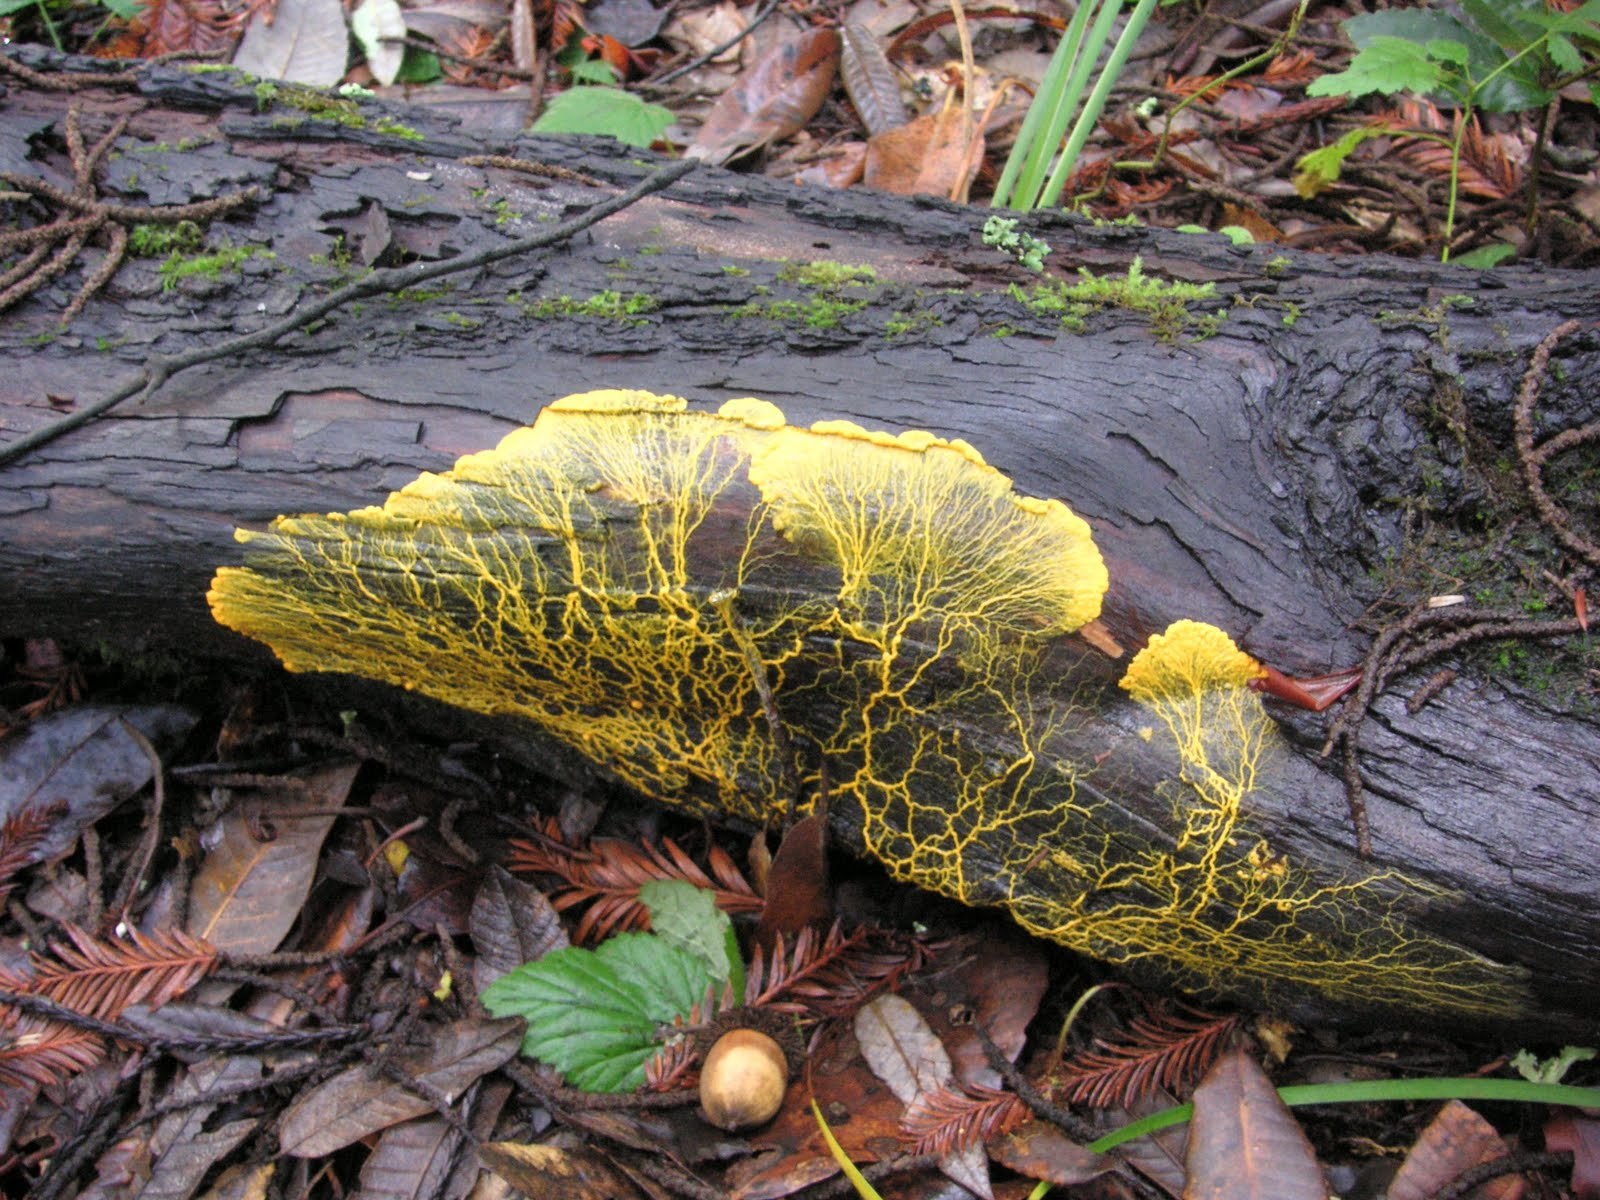
\includegraphics[width=\twoimageswide,keepaspectratio]{physarum_exploring_forest.jpg}\label{fig:exploration:forest}}
		\qquad
		\subfloat[\P exploring the lab][]{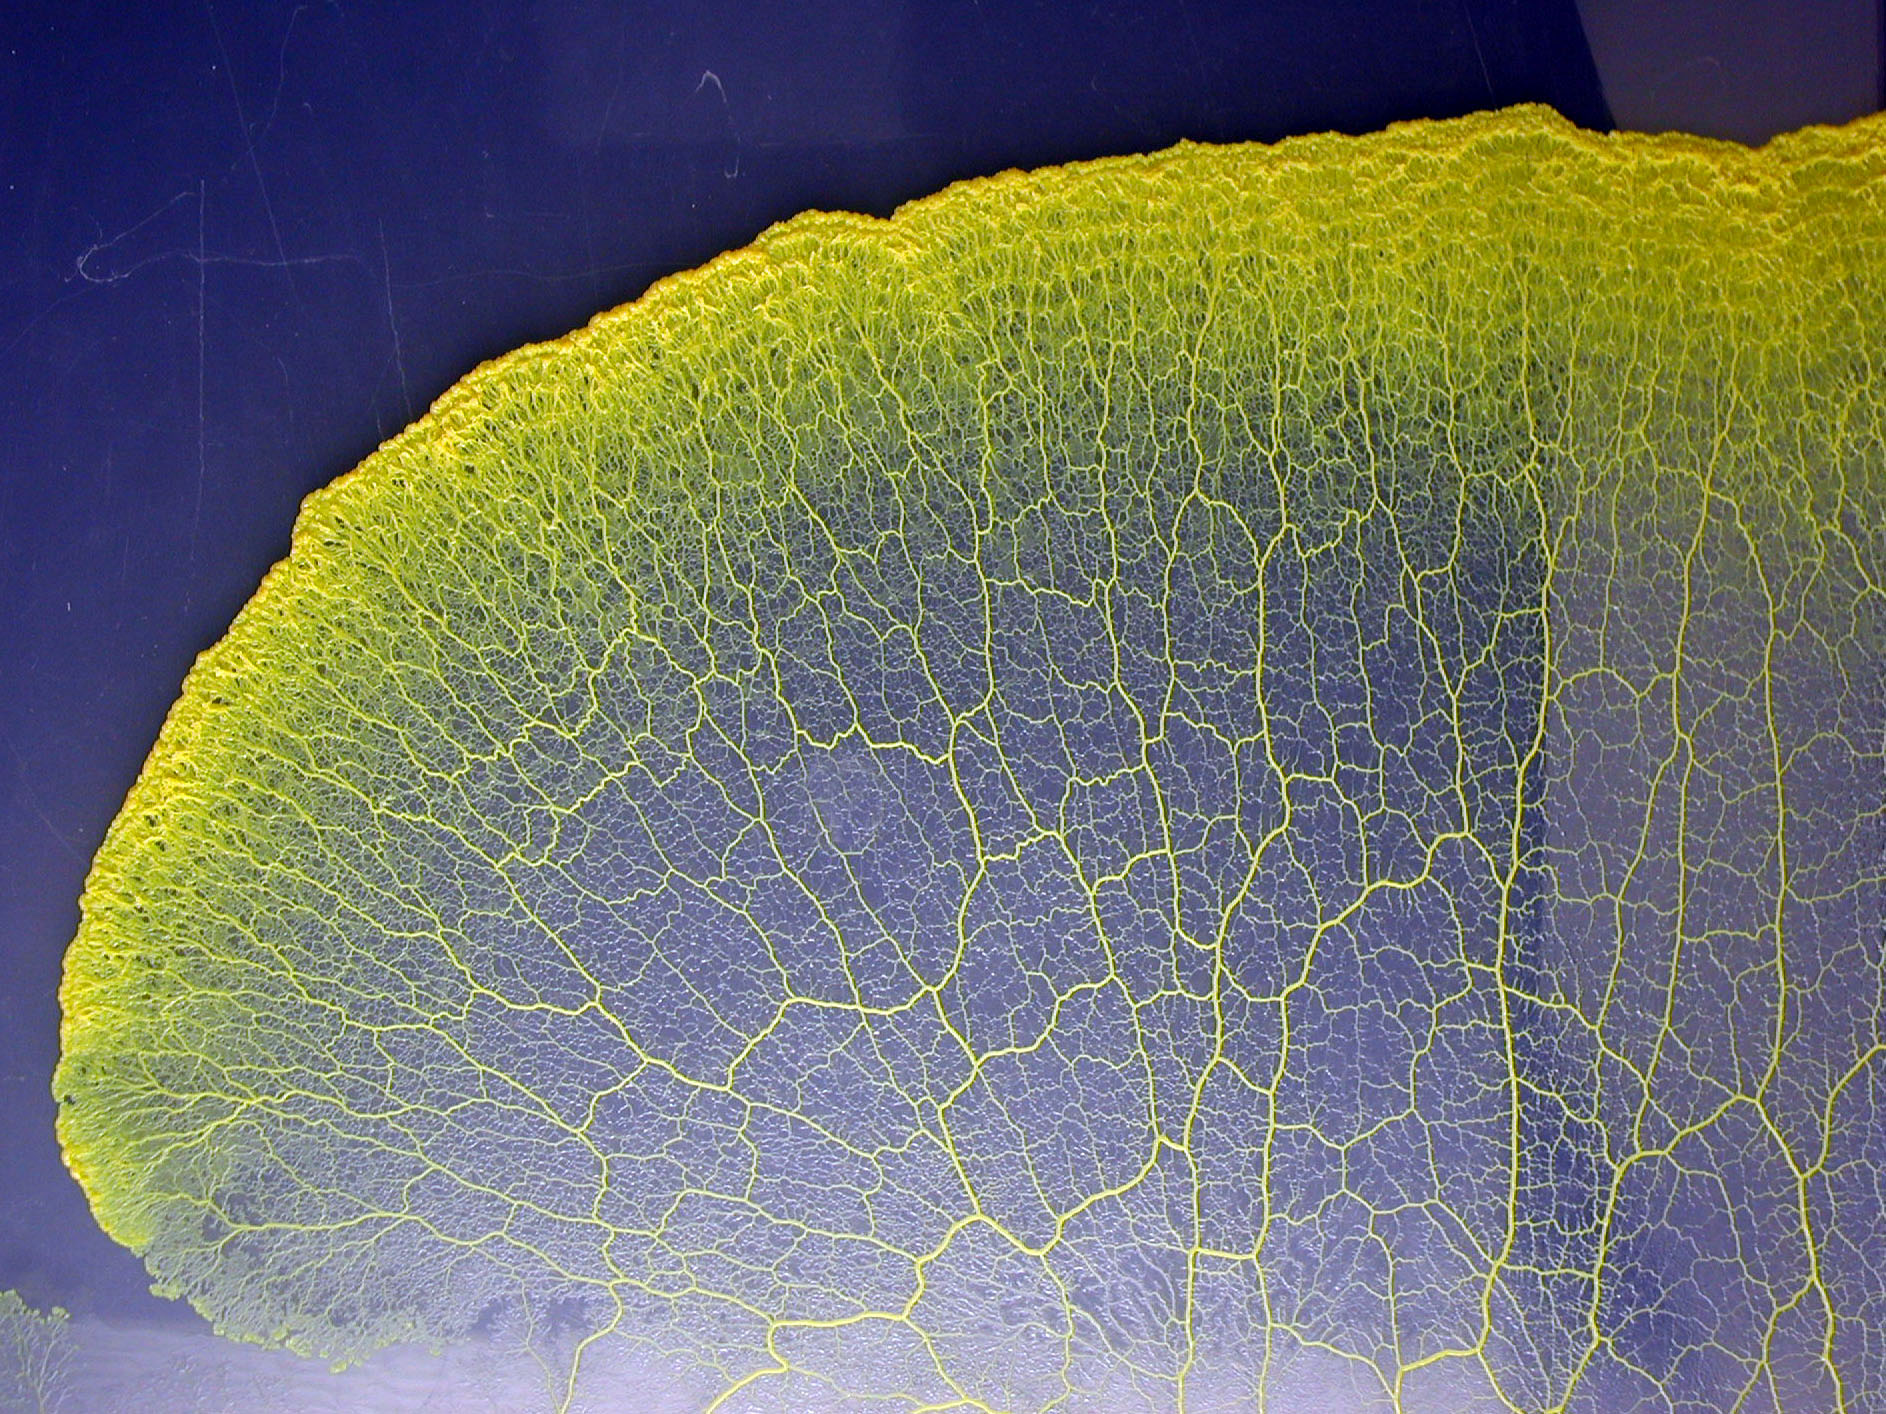
\includegraphics[width=\twoimageswide,keepaspectratio]{physarum_exploring_petri_dish.jpg}\label{fig:exploration:lab}}
		\caption[\P exploring various environments]{Today \P seems equally at home in the forest (a) and the in the laboratory (b). Figures courtesy of Prof.~T.~Ueda, Hokkaido University.}
		\label{fig:exploration}
	\end{figure}

	In the following we give a concise introduction to \Pp, discussing its life cycle and scientific importance. We emphasize the plasmodium stage in particular, which is of key importance for all natural computing applications discussed in \Fref{sec:natural_computing_physarum}. We summarize selected material form several sources which may be consulted for more detailed surveys~\cite{stephenson1994myxomycetes,nowotny2000myxomyceten,grube2016physarum,Sauer1986,Mayne2016,howard1931life}. Our exposition closely follows the structure of~\cite{nowotny2000myxomyceten}.
	
	\FloatBarrier
	
	\subsection{Life of Slime}


		The life cycle of \P starts with its spores which are propagated in a predominately airborne fashion. After an incubation period of a few days, spores begin to germinate given favorable conditions. As a result the walls of the spores break open to release haploid protoplasmic bodies of \SIrange{12}{15}{\micro\metre} in diameter. After a short period of quiescence these so-called myxoamoebae become active to grow and multiply much like other soil amoebae. 

		Two reversible processes illustrate the remarkable adaptability of \P myxoamoebae. First, they have the ability to quickly grow one or two flagellae, \ie change into myxoflagellates. This enables them to better navigate moist environments such as water films. If moist conditions are are followed by dry ones said the organism can change back to its non-flaggelate form.	Second, both types of myxoamoebae may form dormant micro cysts capable of enduring adverse conditions such as exreme dryness or strong illumination. As soon as conditions become favorable again, myxoabmoebae escapte their cysts and are ready to continue the life cycle.

		In the next stage, pairwise sexual or heterothallic fusion between two haploid myxoamoeba are observed. This leads to the irreversible formation of a diploid zygote. It is also possible that a single myxoamoeba changes directly into a haploid zygote in an apogamic or selfing fashion.

		Both types of zygotes have in common that from now on, nuclear division happens synchronously every \SIrange{8}{10}{\hour} without cell devision. This dramatic change signals the onset of a peculiar cellular organization, the so-called \emph{plasmodium}. In this stage \P lives as an macroscopic brightly yellow mass of protoplasm consisting of up to millions of nuclei contained in a singular cell. Remarkably, the plasmodium stage is unique to myxomycetes and unparalleled throughout all of nature.

		In its plasmodium stage \P is acting as an undifferentiated macroscopic creature, capable of sensing food sources, migrating towards them and feeding on them by means of phagozytosis. Typical food sources encountered by \P in the field include bacteria, amoebae, algae, common molds and various organic materials. It is also known to feed on spores, hyphen or fruting bodies of higher fungi. In the lab \P can sustain itself on substrates containing solute nutrients. Under continued food intake, the plasmodium can grow to cover large areas of up to  several \si{\deci\metre\squared}. Under unfavorable conditions the plasmodium can change into many multinucleated dormant macrozysts, forming a crust of dried slime, the so-called \emph{sclerotium}. \P may reverse back to its plasmodium form in better conditions even after prolonged periods of lying dormant. 

		Towards the end of the life cycle, triggered by lillumination, the plasmodium seeks out dry and preferably elevated locations to begin the irreversible process of sporulation. In a synchronus differentiation procees \P forms colonies of \SIrange{1}{2}{\milli\metre} tall fruiting bodies. These so-called sporangia are numerous and come with a stem and a head each. Their appearance inspired its species designation \Pp, the multiheaded. Within the fruiting bodies spores are maturing which are responsible for species propagation. After maturing fruiting bodies break open which allows the contained spores to be dispersed by the wind. Thus the life cycle of \P, given suitable conditions, may start anew.

		It is fascinating how this multipotent development system exists in extremely different forms of live while controlled by one and the same genome in a unique temporal sequence. From spores to amoeba, on to plasmodium and finally to fruiting bodies. From there back to spores and again into more amoeba. The complete life cycle of \Pp is illustrated in \Fref{fig:life_cycle}.

		\begin{figure}[htb]
			\centering
			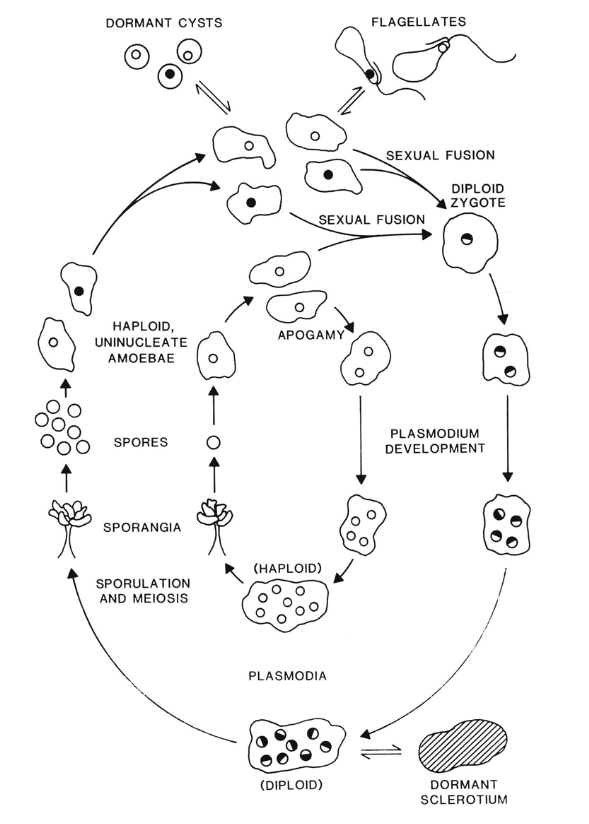
\includegraphics[width=\textwidth,height=0.8\textheight,keepaspectratio]{life_cycle.png}
			\caption[Life cycle of \P]{The complete life cycle of \Pp. Reprint from~\cite{Sauer1986}.}
			\label{fig:life_cycle}
		\end{figure}

		Next we discuss the plasmodium stage of \P in more detail as it is most relevant to \Fref{sec:natural_computing_physarum}.

		\FloatBarrier

	\subsection{The Plasmodium of \textit{P. Polycephalum}}

		The typical plasmodium of \P takes the shape of an extended sheet-like structure capable of moving to explore unvisited territory in search of food sources. \Fref{fig:exploration} illustrates that in this stage of its life cycle, the organism consists of a complex vein network (bottom right area of image) which connects to the boundary of the organism, its apical zone or growing front (arcing from bottom left to top right). \Fref{fig:apical_zone} and \Fref{fig:supporting_network} show details of the apical zone and the vein network respectively. The overall shape of the network is highly dynamic and may change drastically in response to changing environmental conditions such as encountered attractants or repellents. This extraordinary functional plasticity allows \P to navigate its environment successfully.

		
		\begin{figure}[!htbp]
			\centering
			\subfloat[][]{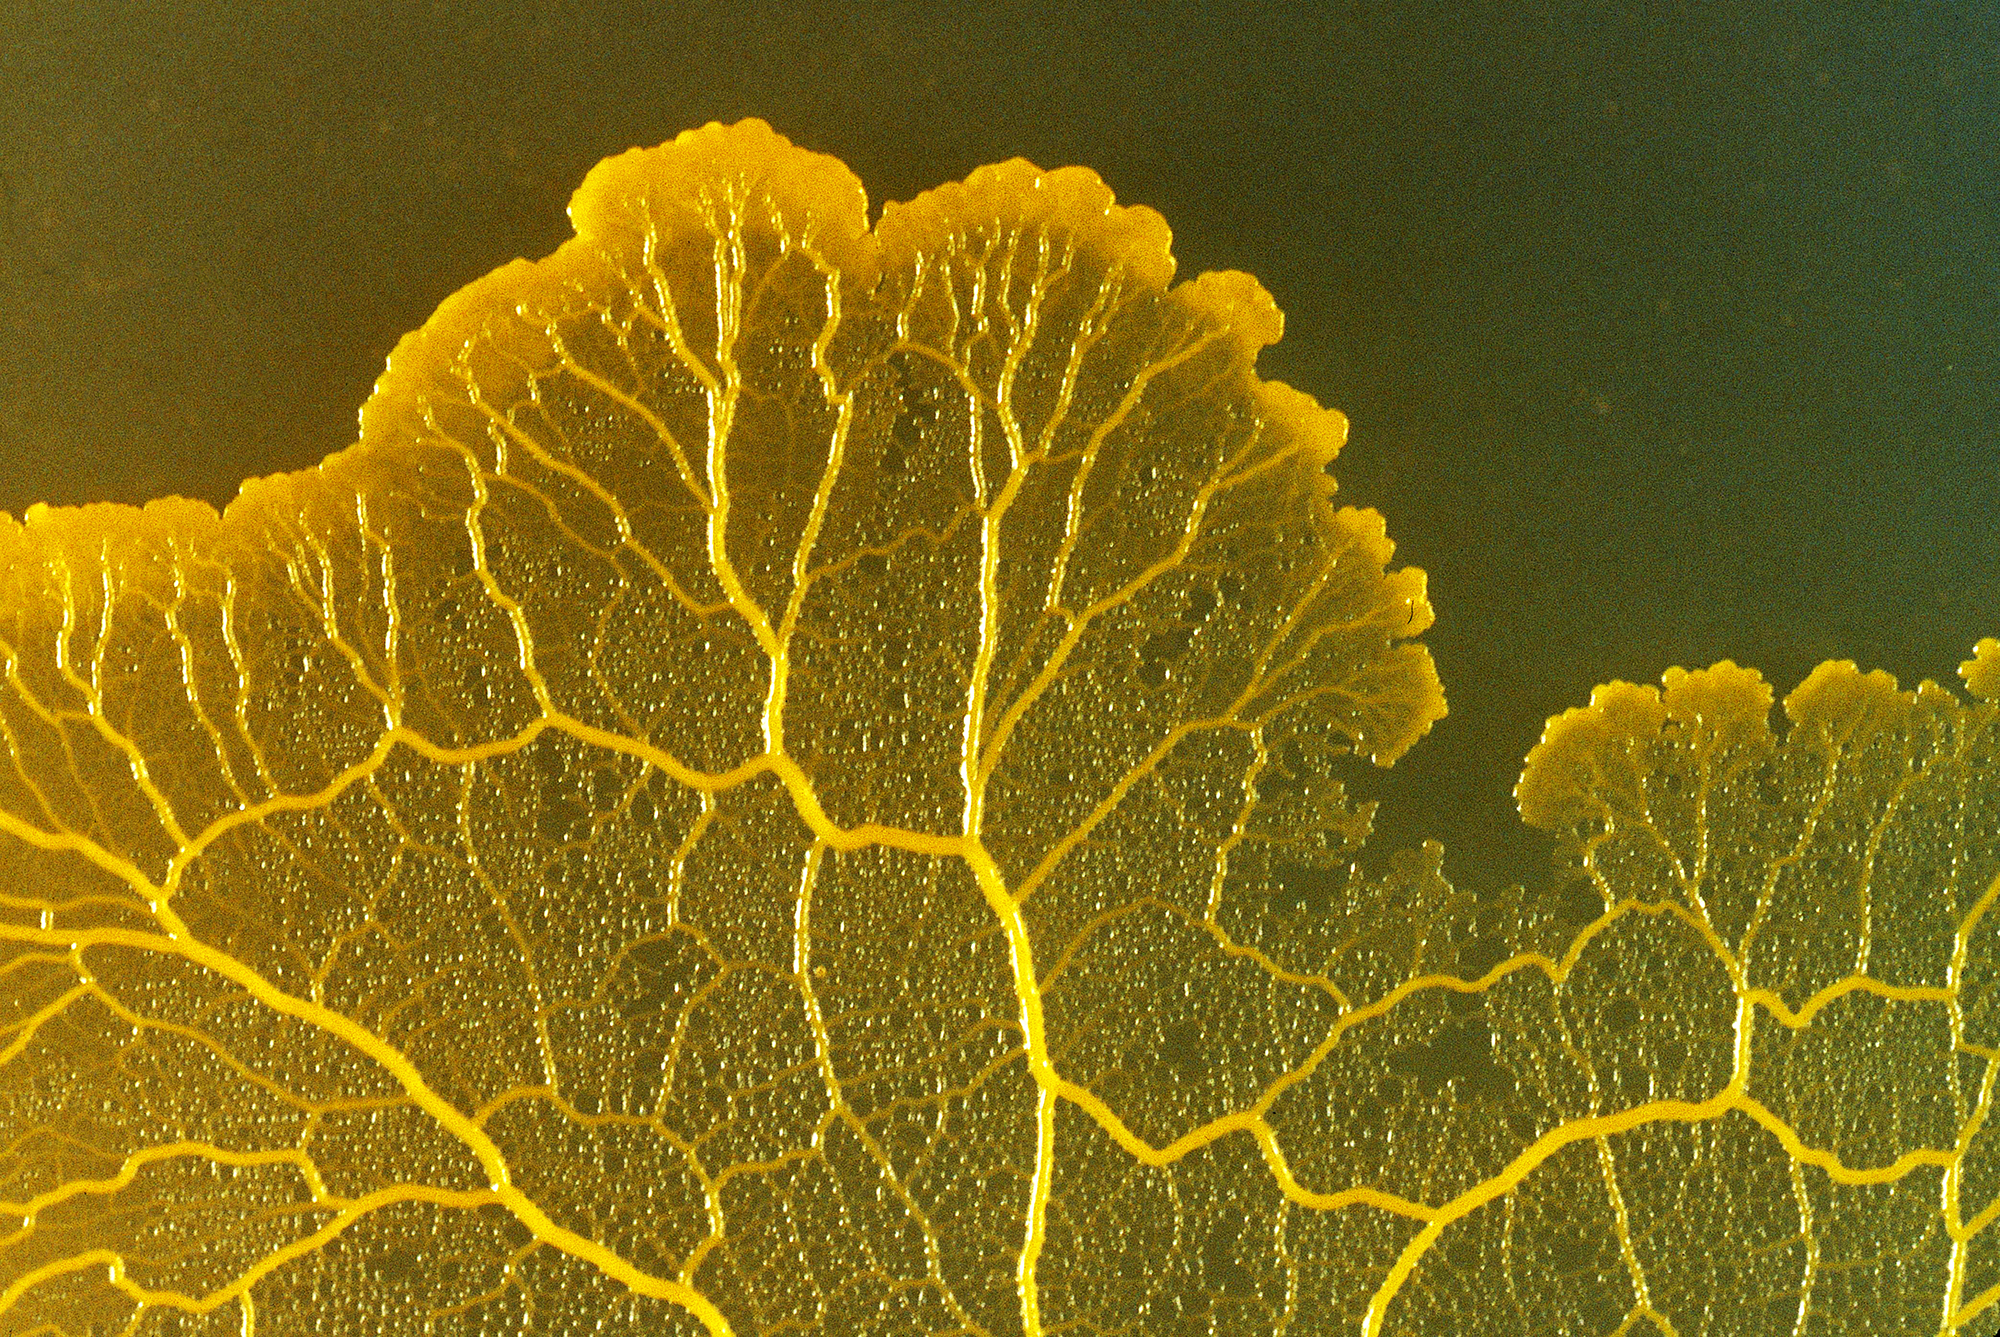
\includegraphics[width=\twoimageswide]{slime.jpg}\label{fig:apical_zone}}
			\qquad
			\subfloat[][]{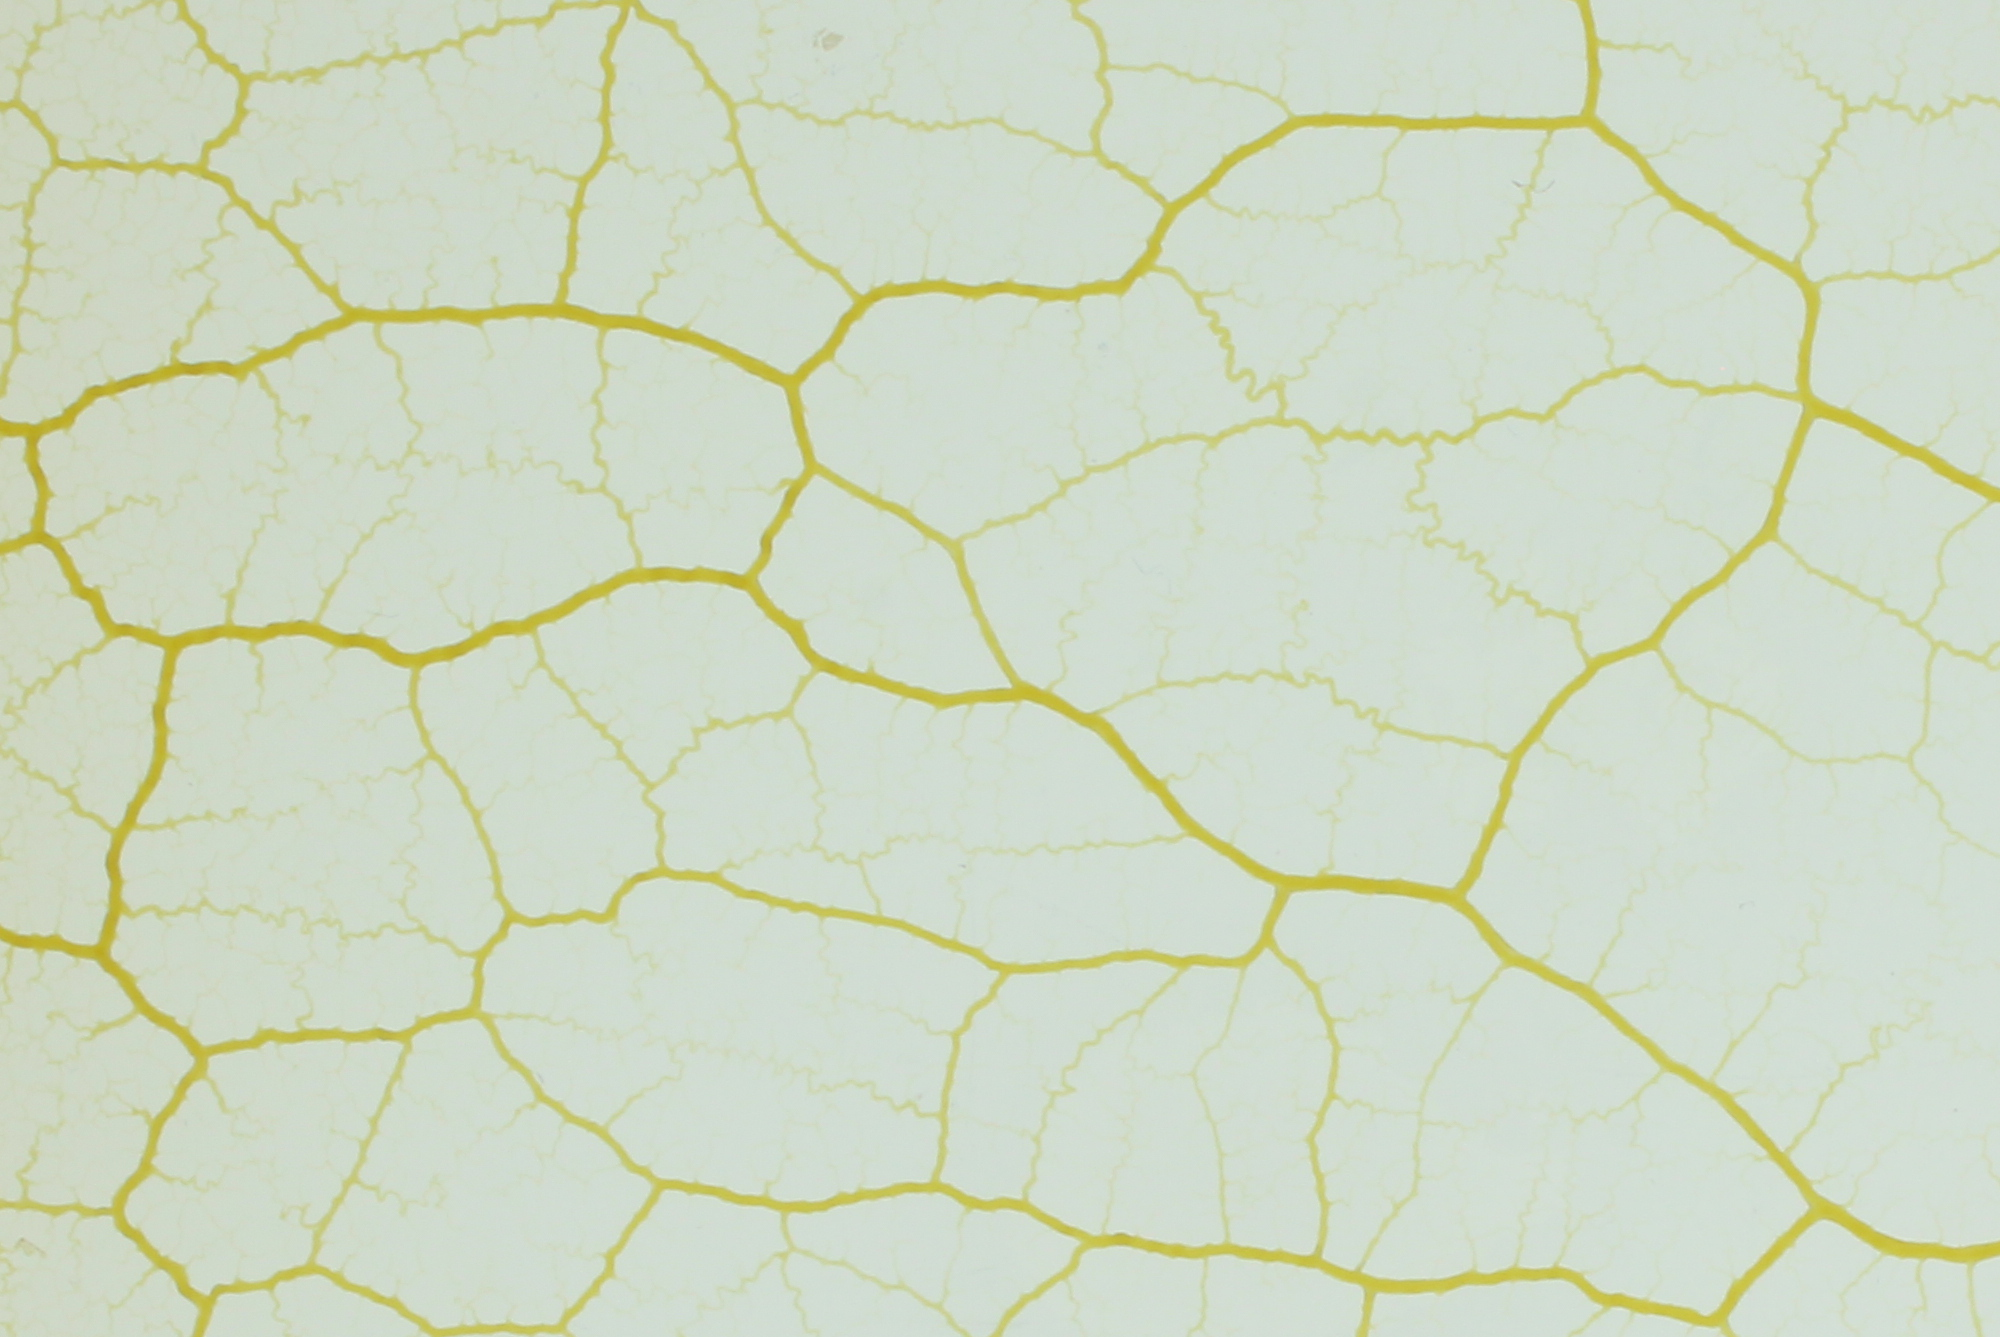
\includegraphics[width=\twoimageswide]{network.JPG}\label{fig:supporting_network}}
			\caption[Details of apical zone and supporting network]{(a) Detailed image of the apical zone being supported by thick veins. (b) A larger example of the complex vein network. Note the large cycles of thick veins. Smaller veins provide additional connections.}
			\label{fig:plasmodium_details}
		\end{figure}

		
	
		The veins themselves which form the tubular network are approximately cylindric with vein walls consisting of a thick connected mesh of actin and myosin fibers. Within the veins protoplasmic fluid, for short protoplasm, can freely flow back and forth, transporting cell nuclei, nutrients and various other relevant materials. \Fref{fig:plasmodium_hand_drawing} shows a schematic drawing of a macro plasmodium.

		\begin{figure}[!htb]
			\centering
			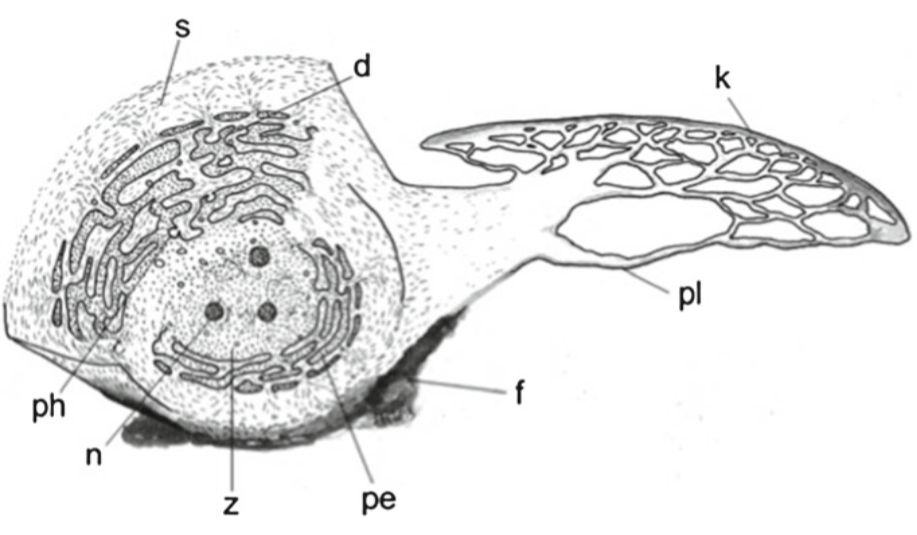
\includegraphics[width=\oneimagewide]{plasmodium_hand_drawing.png}
			\caption[Schematic drawing of the plasmodium of \P]{Schematic drawing of slime mold plasmodium with facing side sectioned and upper left section enlarged. \textbf{\texttt{k}} moving front, \textbf{\texttt{pl}} trailing plasmodial strand, \textbf{\texttt{f}} deposited material, \textbf{\texttt{s}} slime; \textbf{\texttt{d}} vacuole with deposit; \textbf{\texttt{ph}} phagocytosis vesicle; \textbf{\texttt{n}} nucleus; \textbf{\texttt{z}} central plasma; \textbf{\texttt{pe}} peripheric membrane stacks. Peristaltic contractions occur in the peripheric plasma, while the central plasma is subject to shuttle streaming. This figure is hand-drawn by Prof.~M.~Grube, Karl-Franzens Universit\"at Graz. Reprinted with permission from~\cite{grube2016physarum}.}
			\label{fig:plasmodium_hand_drawing}
		\end{figure}

		The protoplasmic flow itself is driven by periodic cross-sectional contractions of the actin-myosin mesh forming the walls of the veins. The contractions realize a peristaltic pumping effect leading to protoplasmic streaming and net material transport. Resulting peristaltic contraction waves can be observed across the entire network inducing complex flow patterns including periodic flow arrests and reversals. Every \SI{50 \pm 5}{\second} the velocity of the protoplasmic flow streaming through a vein decays smoothly until the flow completely arrests. After one or two seconds of standstill, flow velocity quickly accelerates back to normal and the cycle proceeds. Interestingly, after most but not all arrests, the direction of flow is reversed after the flow picks up again. Protoplasmic flow exhibits enormous flow speeds of up to \SI[per-mode=symbol]{1000}{\micro\metre\per\second}\footnote{Flow speeds of \SIrange[per-mode=symbol]{2}{78}{\micro\metre\per\second} known for streaming plasma in plants pale in comparison.}. It is believed that the interplay of network topology, peristaltic pumping and complex flow patterns with high flow velocity facilitates efficient transport of nutrients and signaling molecules across the entire organism. 

		In addition to enabling fluid transport, flow patterns also cause periodic pressure waves arriving at the apical zones of the organism. Each incoming wave extends the organism boundary by a small amount by pushing forward protoplasm that arrives via the vein network. This process is called shuttle streaming. The pressure of the streaming protoplasm is so high, that the material practically shoots out of the supporting veins, causing the fan-like growing tips that can be seen along the boundary of the organism in \Fref{fig:apical_zone}. Since the advancing growing front leaves behind a network of veins, continued support for expansion is ensured.

		Given abundant food supply, \P rapidly advances a coherent and dense apical zone exploring the available space. The growing front proceeds as one large unit following an exploration strategy aptly termed \emph{phalanx}, see \Fref{fig:exploration:lab} or \Fref{fig:apical_zone}. If nutrients are scarce, however, a different strategy is employed and \P tends to grow several separate distinct growing tip each advancing its own substantially smaller growing front. This behavior increases the odds of discovering more distant sources of nutrients. Since branches may react individually to attractants such as food, a more adaptive search can be achieved. Once new food sources are secured, the organism can concentrate its movement towards them by reallocate its mass as needed. This strategy has been termed \emph{guerilla}. \Fref{fig:exploration:forest} shows a separate growing tip on the right side which illustrate that the plasmodium of \P may naturally interpolate between the two extreme strategies. The strategies employed by \P are reminiscent of two well know graph traversal strategies: Breadth-first and Depth-first search. In BSF, the explored region grows uniformly like a wave that expands evenly in all available directions. In contrast to that, DFS choose one direction in order to explore it to maximum depth. Then it backtracks to resolve the places that were ignored so far.

		Finally, we remark that the plasmodium stage of \P can be regarded as simple in terms of its biological organization because it lacks any form of brain or nervous system capable of orchestrating complex tasks such as foraging for food. The fact that the organism still displays a level of complex organized behavior sufficient to survive is one of its most fascinating features. Today it is believed that effective global organization emerges from the delicate interplay of local effects such as periodic contractions, topological dynamics and the integration of environmental signals. Shedding light on the details of these dynamics remains one of the major challenges in \P research.

		\FloatBarrier

	\subsection{Overview of Research Focused on \textit{P. Polycephalum}}

		\P develops exceptionally well when cultured in the lab which makes it an ideal subject for scientific studies. Significant research activity in the beginning of the latter half of the 20th century explored the life cycle of \P and described the morphology and physiology of its various stages for the first time. Culturing procedures as well as genetic and molecular techniques were developed that allowed a detailed study of its mitotic cycle, cellular motility, differentiation and many other questions of biological interest. Although interest in \P was at first exclusively fueled by general questions of Biology, the scientific community soon began to appreciate the value of \P as multi-potent model system that could be controlled and studied effectively. Within a short period \P became a core experimental platform, driving a wide variety of research efforts. The study of cell motility is particularly noteworthy in this context. Relevant reviews dating from the 80th can be found in~\cite{dove1980growth, aldrich2012cell,sauer1982developmental,Sauer1986}.

		After a period of intense efforts up to the 80th, the remainder of the century saw a general decline in interest related to \P. It should not end until the beginning of the 21th century, when exciting new question surrounding the networks formed by the plasmodium of \P arose\footnote{Some members of the research community today have been humorously referring to these events as ``the second coming'' of \P.}. In particular, it was shown that the vein networks formed by the plasmodium of \P exhibit highly localized dynamic oscillatory behavior and a capability to adaptively change their topology. Together with its remarkable chemotactic abilities, these properties play a key role in the foraging behavior of \P. Despite the lack of any centralized control, they enable the organism to act as an organized unit in order to establish robust and effective vein networks connecting a potentially large set of spatially distributed food sources. In a similar context, the vein network established by \P has been shown experimentally to mimic man-made transportation networks such as railway systems or highways~\cite{tero2010rules,tero2006physarum,nakagaki2004smart}. Furthermore, it has been demonstrated that the plasmodium of \P can establish the shortest path between a pair of food sources placed in a maze~\cite{nakagaki2000intelligence}. These astounding feats received major interest amongst scientists of many disciplines and earned \P a place in the perception of the general public. Within a short period of time, \P became the focus of diverse interdisciplinary research efforts, engaging Biologists, Physicists and Computer Scientists alike. The renewed multi-disciplinary interest lead to a resurgence of research in \P that can be observed to date. For a rare, more recent review, and various recent results see~\cite{ueda2005intelligent} and~\cite{takamatsu2009environment,shirakawa2007emergence,alim2013random,tero2007mathematical,nakagaki2004obtaining}. Please note that this selection represents a fairly limited part of current research on \P. In fact, it is focused on results revolving around the network forming plasmodium stage of \P which are relevant in the context of this thesis.

		\FloatBarrier

%!TEX root = ../../../../thesis.tex
\section{Natural Computing}\label{sec:natural_computing}

	For some time the words \emph{Nature} and \emph{Computing} used to denote terms which could hardly be any more opposite to each other. Starting in the mid 1940s this perception began to fade gradually when researchers started to explore the exciting possibility of looking towards nature for alternative ways of doing computing. The search for new problem solving techniques, novel approaches to synthesize natural phenomena \emph{in silico} as well as novel natural materials capable of realizing computations began. Today, the pursuit of these three distinct, yet interrelated approaches is known as \emph{Natural Computing}~\cite{de2005natural,de2006fundamentals}.

	In this section we give a short introduction to the scope of natural computing and mention its most important areas of interest. Our exposition closely follows de~Castro~\cite{de2007fundamentals}, who describes natural computing as the extraction of ideas from nature to develop computational systems, or using natural materials to perform computation. He suggests to divide the field into three main areas:

	\begin{description}
		\item[a)] Computing inspired by nature
		\item[b)] The simulation and emulation of nature by means of computing
		\item[c)] Computing with natural materials
	\end{description}

	\begin{figure}
			\centering
			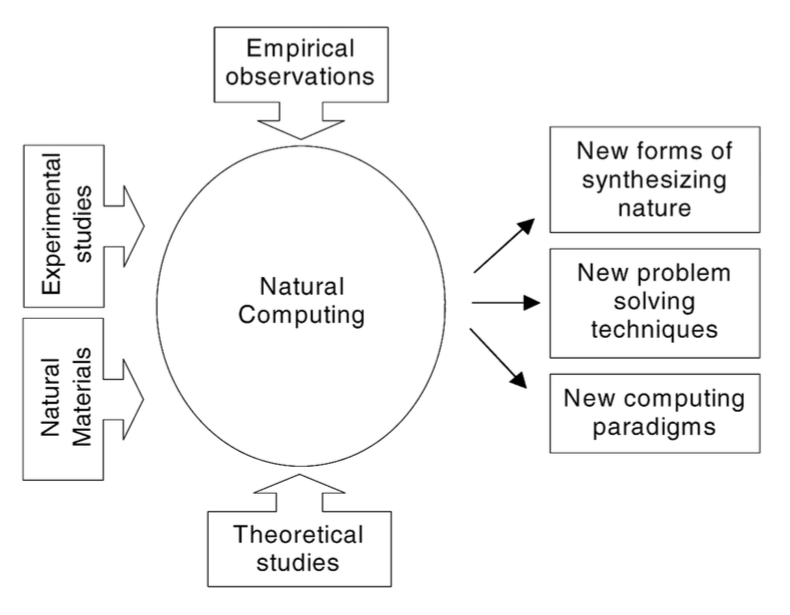
\includegraphics[width=\oneimagewide,keepaspectratio]{natural_computing.png}
			\caption[The goals of natural computing.]{A schematic of the components and goals of natural computing.}
			\label{fig:natural_computing}
	\end{figure}

	\Fref{fig:natural_computing} illustrates the goals of natural computing. The study of these three highly entangled areas seamlessly merge empirical observations and theoretical studies from diverse fields such as biology, physics, chemistry, engineering and computer science amongst others. Thus it is vital for researchers to be open, collaborate and share their ideas and knowledge in order to meet the challenges posed by the highly interdisciplinary field that is natural computing.

	What follows is a short description of the main areas of natural computing including some of its most important achievements. For an extensive discussion and a comprehensive collection of references see~\cite{de2007fundamentals}.

	\FloatBarrier

	\subsection{Computing Inspired by Nature}

		In the area of natural computing, the goal is to utilize natural processes and phenomena as a source of inspiration in order to devise novel computational systems and algorithms geared towards solving complex problems. Of particular interest are alternative solution methods for problems for which standard techniques such as linear, non-linear and dynamic programming encounter severe difficulties. Some of the best known representatives of nature inspired computing include artificial neural networks\footnote{The field of artificial neural networks deals with computational problems as opposed to the accurate biological modeling of the brain and the nervous system. The latter are questions of computational neuroscience.}, evolutionary algorithms and swarm intelligence~\cite{de2007fundamentals}.

		\newpage

		\begin{description}
			
			\item[Neural networks] are formed by \emph{artificial neurons} arranged according to a predefined network architecture, typically consisting of several functional layers of neurons. Triggered by a special \emph{activation function}, each neuron may fire, \ie mapping its potentially many weighted inputs to a single output. Different types of \emph{learning strategies} may adjust the input weights of each neuron in response to encountered input stimuli. Indeed, some amount of learning, also known as training, is typically required before a neural network becomes competent. Given proper training various problems such as classification, pattern recognition or more general function approximation can be solved without further assisting the neural network. Unfortunately, a deeper understanding of why neuronal networks work the way they do remains elusive. A fact, that does not diminish their usefulness which lead to their large (commercial) success. For references see~\cite{Haykin:1998:NNC:521706,Fausett:1994:FNN:197023,Bishop:1995:NNP:525960}.

			\item[Evolutionary Computing] and in particular genetic algorithms, try to leverage the power of evolution by simulating a population of individuals with certain traits. Individuals represent points in a search space associated with solutions to a given optimization problem. Each potential solution is evaluated with regards to the objective function of the problem. This process is known as determining the \emph{fitness} of an individual. Individuals are then selected to reproduce, \ie pass on their traits to the next generation, with a probability proportional to their fitness in an sexual or asexual fashion. In the former case the offspring is determined by a recombination of the traits of the parents. Further genetic variation is introduced by random mutation of traits. If this process is repeated, it evolves towards better solutions in an iterative manner. Typically such algorithms terminate after a predefined number of iterations or when the desired level of fitness is reached. Evolutionary algorithms have found success in problems such as routing, scheduling, packing and various machine learning tasks~\cite{Back:1997:HEC:548530,spears1993overview,zitzler2000comparison}. Important practical applications include determining optimal design choices in various engineering settings~\cite{Schwefel:1993:EOS:529401,kicinger2005evolutionary}.

			\item[Swarm Intelligence] encompasses techniques for problem solving that are inspired by the collective behavior of human or animal societies. They rely on the social behavior of a population of individuals capable of interacting with the environment or one another in either a direct or indirect fashion~\cite{de2007fundamentals}. The popular \emph{ant colony optimization} approach uses artificial ants that lay and follow artificial \emph{pheromone trails}. In the shortest path problem for instance, ants travel all possible paths between two distinct nodes at the beginning. However, as time goes by, longer routes have less pheromones associated with them due to pheromones evaporating. Since the probability for an ant to choose a given route is proportional to the present amount of pheromone, ants become less likely to travel long routes and tend to concentrate on the shorter paths, thereby reinforcing them repeatedly. As a result, ants are progressively converging towards the shortest path. This general scheme can be adapted to various other discrete optimization problems such as the traveling salesman problem and certain vehicle and network routing problems. For references see~\cite{bonabeau2000swarm,bonabeau2000inspiration,Bonabeau:1999:SIN:328320,fukuyama2008fundamentals}.
			
		\end{description}

		\FloatBarrier

	\subsection{Synthesis of Nature by Means of Computing}
		
		The synthesis of nature by means of computing aims for full or partial reproduction of phenomena, behaviors or patterns observed in nature~\cite{de2007fundamentals}. This \emph{in silico} approach allows the exploration of a wide range of questions which may not be tractable using traditional analytic or experimental techniques. Frequently theoretical work suggest theories and models to be studied \emph{in silico} using simulations with the aim of obtaining a deeper understanding of the original phenomenon being modeled. The simulation itself may serve as an evaluation of a proposed model, ideally suggesting further improvements to the model and itself. In addition to the sheer growth in computing power observed in the last few decades, much of the success of fields like computational biology, computational chemistry or computational physics owes to the symbiotic relationship between theory and simulation.

		Examples for the synthesis of natural phenomena include \emph{cellular automata} as a model for self-reproduction or \emph{L-systems} modeling the development of multicellular organisms. These concepts were designed to capture and study certain, well-defined rules and associated behaviors. However, over time their elegance and simplicity lead to a variety of unforeseen applications. Cellular automata have played a role in modeling the physics of fluids or gases on lattices~\cite{rothman2004lattice}, and the microscopic study of high-way traffic~\cite{nagel1998two}, to name but a few. L-systems have been a successful tool in the study of various properties of \emph{virtual plants}~\cite{tardieu2003virtual}. In addition to that they have found applications outside of biology in formal language theory, the study of tumor growth and even musical composition~\cite{de2005natural}.

		Arguably the most exciting field we like to mention in the context of synthesis by means of computing is the study of \emph{artificial life}~\cite{Langton:1995:ALO:526815}. Within artificial life, it is proposed that life itself should be regarded as an emergent property resulting from the organization of matter as opposed to a simple property of matter itself. It follows that besides the carbon based chain of life observed on earth, \ie \emph{life-as-we-know-it}, different materials could lead to alternative life-like organizations aptly termed \emph{life-as-could-be}. While it is debatable what properties such an organization requires to be rightfully termed \emph{alive}, the prospect of new unknown forms of life is extremely exciting. 

		A well-known example for non-trivial behavior in the context of life-as-could-be is demonstrated by \emph{boids}~\cite{Reynolds:1987:FHS:37401.37406}. Here artificial life is represented merely as virtual agents that are allowed to move in space. They obey the following simple rules: (1)~Avoid collision with neighboring boids or obstacles; (2)~Mirror velocity and direction of neighboring boids; (3)~Stay close to neighboring boids. From these simple rules complex collective behavior emerges allowing a flock of boids to closely imitate the non-trivial behavior seen in flocking birds or shoals of fish~\cite{de2007fundamentals}.

		The examples in this section illustrate that much can be learned from attempts to synthesize nature by means of computing. It is likely that ongoing research efforts will sooner or later drastically alter our understanding of nature in general and life in particular. It is this authors personal opinion that the question of how life arises from inanimate matter constitutes one of the most important scientific questions in the entire history of science.

		For extensive reviews on the topic of artificial life, we refer the reader to~\cite{Langton:1995:ALO:526815,Boden:1996:PAL:525139,bedau2000open,taylor1993artificial}.

		\FloatBarrier

	\subsection{Computing with Natural Materials}

		Computing with natural materials aims to go beyond standard transistor-based computing by utilizing natural materials other than silicon as media for computing. Examples for approaches to computing that are in stark contrast to conventional computing are DNA and quantum computing~\cite{de2007fundamentals}. 

		In \emph{DNA computing} complex molecules such as DNA strands are used to store and process information. Complex computations can then be realized using a set of basic operations that apply to interacting molecules. These operations are derived from molecular biology and involve fusing, copying or deletion of DNA strands to name but a few. The power of DNA computing derives from the fact that a large number of molecules may interact with each other simultaneously. Despite the potentially slow individual reactions, the inherent massive parallel information processing capability of DNA computing lead to novel approaches to hard combinatorial problems such as the Hamiltonian path problem~\cite{adleman1994molecular}. Today various other applications are known ranging from matrix multiplication to cryptography~\cite{puaun2000computing,boneh1996computational,lipton1996breaking,oliver1998computation}. Drawbacks of DNA computing include scaling with problem size as well as retrieving the actual problem solution from the DNA computation~\cite{de2007fundamentals}.

		Another promising alternative to classical computing is \emph{quantum computing}~\cite{Nielsen:2011:QCQ:1972505}. Here the so-called \emph{qubit} replaces the classic binary bit which is limited to the two states, $0$ or $1$. In contrast to that, the qubit, thanks to its quantum nature, can represent any superposition state of the classical bit states. Thus it is capable of representing all possible combinations of $0$ and $1$ \emph{simultaneously}. As a result, a quantum computer using $n$ qubits may be in $2^n$ different states at the same time, very much unlike a classical computer which is in exactly one state at a time. 

		Elementary operations on qubits take the form of quantum logic gates. Gates may be arranged in such a way that they compute the solution to a given problem. A sequence of gates operating on qubits is then called a \emph{quantum algorithm}. In the final steps of any quantum algorithm the qubit superposition is collapsed in order to obtain the result which is often probabilistic in nature. Exploiting the massive in-build parallelism, dedicated quantum algorithms have been developed that outperform all known classical algorithms for a small set of problems. The two most prominent ones being Shor's integer factorization and Grovers's database search algorithm~\cite{shor1999polynomial,grover1996fast}. 

		In addition to speeding up certain tasks, quantum systems may operate in ways that classical systems cannot. This fact is exploited in \emph{quantum communication} or \emph{quantum cryptography}, where protocols have been developed which reduce communication complexity or provide perfect secrecy~\cite{de2007fundamentals}. A major roadblock on the way of success for quantum computing consists of the physical realization of coherent systems capable of preparing qubits and executing quantum algorithms reliably. Here the very quantum nature which enables extraordinary computation, presents formidable difficulties when it comes to controlling the quantum system. Unfortunately this fact still severely limits the number of qubits that have been used in successful computing applications~\cite{Nielsen:2011:QCQ:1972505}. 

		\FloatBarrier

%!TEX root = ../../../../thesis.tex
\section{Natural computing with P. Polycephalum}

	It can be argued that a necessary precursor to \P being discovered as a suitable substrate for natural computing consist of a series of break-through experiments of Nakagaki et al. that changed our perception of the unassuming organisms that are slime molds.
	
	The first of which was introduced in the year 2000. In the so-called ``maze experiment'' the plasmodium of \P is introduced to a maze, see \Fref{fig:maze:initial}~\cite{nakagaki2000intelligence}. After the plasmodium has spread evenly across the entire maze, two food sources are introduced at two specific points in the maze, see \Fref{fig:maze:intermediate}. The organism forms veins while slowly retracting from areas of the maze that do not intersect with any path connecting the two food sources. This process continues until the plasmodium takes the shape of one single thick vein connecting the food sources. In repeated experiments, it was shown that the organism occupies precisely the shortest path ($\alpha_1 + \beta_1$) in most of the cases. This demonstrates the organisms remarkable ability of iteratively improving the connection between the two food sources.
	In this context an improvement is achieved if veins become either shorter or wider in diameter. Since nutrient transport is subject to hydrodynamic forces, shorter and wider tubes entail less resistance to fluid flow~\cite{kamiya1959motive}.

	One may interpret the maze as a graph with edge weights equal to the lengths of the associated maze segments and the food sources as two distinct nodes $N_1$ and $N_2$, see~\Fref{fig:maze:abstraction}. Thus the slime mold \Pp can be seen to demonstrate a solution to the $s-t$ shortest path problem with $s=N_1$ and $t=N_2$.

	\begin{figure}
		\centering
		\subfloat[Maze experiment - Initial state][]{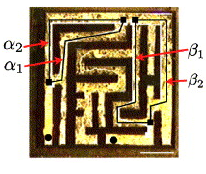
\includegraphics[width=0.45\linewidth,keepaspectratio]{maze/maze_experiment_1.png}\label{fig:maze:initial}}
		\subfloat[Maze experiment - Intermediate state][]{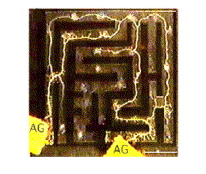
\includegraphics[width=0.45\linewidth,keepaspectratio]{maze/maze_experiment_2.png}\label{fig:maze:intermediate}}
		\newline
		\subfloat[Maze experiment - Final state][]{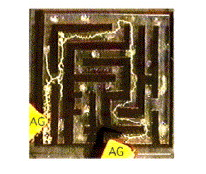
\includegraphics[width=0.45\linewidth,keepaspectratio]{maze/maze_experiment_3.png}\label{fig:maze:final}}
		\subfloat[Maze experiment - Graph abstraction][]{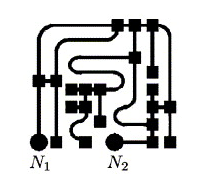
\includegraphics[width=0.45\linewidth,keepaspectratio]{maze/maze_experiment_4.png}\label{fig:maze:abstraction}}
		
		\caption[Classic maze experiment with \P]{ a) The plasmodium of 
		\P is evenly spread across a maze. Filled black circles denote two specific points in the maze. Arrows indicate segments of possible paths between them. b) Two food sources (AG) are introduced at the specific points. After a while the plasmodium retreats from areas of the maze that do not intersect with a path connecting the food sources. c) The plasmodium settles on the shortest path between the two food sources. d) The maze can be interpreted as an abstract graph with two distinct nodes $N_1$ and $N_2$ corresponding to the food sources. The scale bars denote 1 cm. Reprinted from~\cite{Tero2007553}.}
		\label{fig:maze}
	\end{figure}

	In 2004 \P was presented with three or more food sources arranged in a regular pattern~\cite{nakagaki2004obtaining}. In repeated experiments the organism was found to connect the food sources in patterns that frequently resemble well known structures such as minimum spanning trees and minimum steiner trees. The experimenters reported two empirical observations that seem to play a key role in the formation of \P networks: First open-ended or dead-end veins are likely to disappear as time goes by. And second, when more than one vein connects the same pair of food sources, all longer veins tend to disappear while the shortest vein is reinforced. 
	
	These observations have been explained on a physiological level in~\cite{Tero2006115}. The plasmodium of \P organizes itself through the formation of thick veins through which the protoplasm is driven as a result of periodic contractions of the veins themselves, \ie peristaltic pumping. The veins are formed if streaming of protoplasm persist in a given direction for a sufficiently long time~\cite{nakagaki2000interaction}. On a molecular scale Actomyosin fibers carried by the protoplasmic flow attach along the lengths of a vein resulting in tubular structures. The fast flowing protoplasm also causes shear stress, exerting a force which stretch-induces a regular orientation of the Actomyosin fibers. As a result, veins with a large flux manage to accumulate and orient additional Actomyosin fibers which over time leads to an increase in vein diameter. This in turn further reduces the resistance to flow because under the assumption that the fluid flow in the veins of \P is a Poiseuille flow, the theory of hydrodynamics dictates that it be proportional to the forth power of the vein diameter and inverse proportional to the vein length. It follows that veins that are carrying little flow either because they are long and/or thin or happen to be dead-end veins are likely to degenerate over time as experimentally observed above. At the same time, reinforcing thick and short veins ensures efficient fluid flow, which in turn enables effective circulation and transport of nutrients, nuclei and signaling molecules.

	These considerations became the basis of a concise model presented in 2006, which captures the behavior of the slime mold as demonstrated in the maze experiment and lead to the first natural computing approaches based on \P~\cite{Tero2006115}. The model can be formulated on a graph $G = (V,E)$, where the node set $V$ denotes the junction points of veins and the edge set $E$ denotes the veins themselves. Each node $u \in V$ has a hydrodynamic pressure associated with it denoted by $p_u(t)$. Each edge $e = (u,v) \in E$ has a length $L_e$ as well as a time-dependent flow through the vein $Q_e(t)$. Here it is assumed that the flow is a Poiseuille flow such that

	\begin{equation}
		Q_e(t) = \frac{\pi r_e(t)^4}{ 8 \eta} \frac{p_u(t)-p_v(t)}{L_e}
		\label{eq:flow_initial}
	\end{equation}
	
	holds. Here $r_e(t)$ is the diameter of an edge and $\eta$ refers to the viscosity of the protoplasmic fluid. Let $D_e(t) = \pi r(t)^4/ 8 \eta$. Then we can simplify \Fref{eq:flow_initial} to read

	\begin{equation}
		Q_e(t) = \frac{D_e(t)}{L_e} (p_i(t) - p_j(t)).
		\label{eq:flow}
	\end{equation}

	Let us choose two distinct nodes $s, t \in V$ representing the source and sink nodes in the graph. Using this definition we obtain an equation for each edge $e \in E$:

	\begin{equation}
		\sum_{e = (u,v) } Q_e(t) =
		\begin{cases}
		\quad 1 & \ \text{for} \ u=s, \\
		\quad -1 & \ \text{for} \ u=t, \\
		\quad 0 & \ \text{otherwise}.
		\end{cases}
		\label{eq:conservation_of_flow}
	\end{equation}
	Note that the l.h.s is chosen such that flow is conserved everywhere except at the source and the sink where flow is entering respectively leaving the graph. Thus one unit of flow is introduced to the system. \Fref{eq:conservation_of_flow} can be solved to obtain the values of the $Q(t)_e$ and the $p_u(t)$ simultaneously.

	Finally the time-dependence of $D(t)_e$ is choose such, that the positive feedback between $D(t)_e$ and $Q_e(t)$ is as described above. For each $e \in E$ the dimensionless equation for $D(t)_e$ reads

	\begin{equation}
		\frac{d}{dt} D_e(t) = f( Q(t)_e ) - D_e(t),
		\label{eq:evolution}
	\end{equation}
	which is called adaptation or \emph{evolution equation}. Here $f$ is a monotonically increasing continuous function such that $f(0) = 0$. \Fref{eq:evolution} is the key of the model which formalizes the experimental observations reported earlier. If at time $t$the flux through an edge is such that $f(Q_e(t)) < D_e(t)$ then $D_e(t)$ decreases which further reduces the flux through $e$. In this scenario an edge $e$ is degenerating. Likewise $f(Q_e(t)) > D_e(t)$ leads to an increase in $D_e(t)$ which further increases the flux. In this case $e$ is reinforced. Only ,$f(Q_e(t)) = D_e(t)$ enables a stationary state which leaves $D_e(t)$ and $Q_e(t)$ constant. 

	The model thus evolves the thickness of veins in \P according to \Fref{eq:evolution} relying on the values of $p_u(t)$ and $Q_e(t)$ which are governed by \Fref{eq:conservation_of_flow}. For suitable choices of $f(Q_e)$ this system can be discretized and solved numerically~\cite{Tero2006115}. For the graph depicted in~\Fref{fig:maze:abstraction} a stationary state was found where the $D_e(t)$ of all edges that do not belong to the shortest path between $s=N_1$ and $t=N_2$ vanished. At the same time $D_e(t)$ of the edge on the shortest path approached a constant. That is, just like the slime mold, the model has selected the shortest path in the graph connecting $s$ and $t$. 

	After this initial demonstration of the viability of \P as a medium for natural computing, computer scientists shortly thereafter started to analyze the model and its variants contributing a sequence of convergence proofs and complexity bounds. For suitable choices of $f(Q_e)$ convergence was proven for planar graphs at first~\cite{miyaji2007mathematical,miyaji2008physarum}, but shortly thereafter proofs were extended to general graphs for the original model and for variations thereof~\cite{Bonifaci2012121,bonifaci2013physarum,ito2011convergence,becchetti2013physarum}. The fact that the theoretical properties of the so-called \emph{Physarum solver} are rather well understood is a rarity amongst natural computing algorithms.

	

	The introduction of the physarum solver also triggered dedicated research efforts aimed at exploring the computational abilities of the slime mold further. The foraging behavior of \P was used in conjunction with several food sources to approximate structures such as minimum spanning trees, steiner trees or voronoi diagrams. More abstract experimental setups were constructed capable of exploiting the light-avoiding behavior of \P to solve small instances of the Travelling Salesman problem. 

	Efforts of harnessing these and other experimental demonstration in the form of models suitable for computation were pursued at the same time. One approach consists of modifying or repeatedly applyign the physarum solver in order to deal with several food sources. This has lead to algorithms that are capable of approximating the steiner minimum tree~\cite{6684158}, max flow, variations of the shortest path problem or physarum based network centrality.

	A second successful approach consists of modelling the behaviour of \P based on a particle swar model. In this model independent agents interact accroding to certain rules which lead to the emergence of global behaviour that resembles \P. This model is very flexible and was used to provide solutions to a range of problems including \todo[inline]{examples here \dots}.

	The disadvantages of these approaches are that the simulation of slime mold behavior in order to obtain a solution as often computationally expensive, even on small graphs. For these reason most algorithms are not competitive in terms of runtime when compared with existing algorithms. 

	However, the true merit of the natural computing lies in the fact that it pioneers a new paradigm of solving old problems. This in turn allows for a fresh approach leading to interesting new questions. While more efficient algorithms for a certain problem may already exist, it is not excluded that a natural computing approach based on \P or other media, yields a solution to some problem that has resisted efficient resolution up until now.



%!TEX root = ../../../../thesis.tex
\section{Motivation for this thesis}

	After introducing the most important experimental facts about \P and discussing the natural computing strategies that followed, we are now in a position to give the motivation of this thesis. Recall for a moment that the most successful approaches focus on capturing the morphological changes observed in \P. The physarum solver for instance replicates the changing  diameter of veins while the multi-agent approach that was discussed aims at mimicking the network topology in a dynamic manner. What these and other approaches have in common is that they are not able to capture another highly distinguishing feature of the slime mold: the periodic reversal of the direction of protoplasmic flows through veins. This feature is highly interesting for several reasons. 

	From a biophysical point of view it can be assumed that flow reversals are a product of the organisms efforts to keep the protoplasmic fluid circulating throughout the whole organism by means of organized peristaltic pumping. An efficient circulation of protoplasm likely is necessary for \P to survive since it ensures that nutrients, nuclei, signaling molecules \etc are equally available across the entire slime mold. Note that such a circulation is naturally maintained despite the dynamically changing and growing underlying network of veins. Also,note the fact that \P lacks any form of nervous system or brain. As a result, there is no central control responsible for coordinating a global circulation. This implies that the circulation of flow is organized in a fully distributed manner.

	From a computing point of view these properties are highly interesting. Phrased otherwise, what \P is naturally doing constitutes a way of approximating or obtaining a solution to the problem of routing resources in a dynamically changing graph. This is an interesting and complex problem with various practical applications which has been studied by computer scientists in the past. Obtaining an algorithm for this problem inspired by \Pp is thus desirable. One may aim to find a new algorithm with the following properties:

	\begin{itemize}
		\item the algorithm maintains a dynamic circulation of flow including flow reversals. Since resources are transported with the flow, they are distributed everywhere.
		\item the algorithm is robust against changes in topology. Neither natural changes of network topology nor accidental disconnection of veins renders the process in a state from which it cannot recover.
		\item the algorithm is distributed and requires no central control. As a result, complex global coordination of any sort must emerge from local interactions.
		\item the algorithm is efficient, which can be assumed given that \P was able to survive up until now.
	\end{itemize}

	Working towards such an algorithm inspired by \P, which covers as many of these properties as possible, constitutes the motivation of this thesis. Our approach implies a sequence of preliminary steps. 

	First and foremost, we aim to find an model which yields a circulating flow including flow reversals for individual edges as displayed by \P. Ideally, this model covers the properties listed above and can be used to derive an efficient algorithm which mimics the way \P distributes resources all across its network of veins by means of peristaltic pumping. 

	The past has shown that successful modeling of natural phenomena approaches tend to build upon a reliable body of experimental data and results concerning the same. This serves two purposes. First experimental results help build intuition which is crucial in the formulation of models. Second, experimental data can be used after models and/or algorithms have been derived to asses the degree of which they resemble the workings of the natural phenomenon in question. Thus, before engaging in attempts to model the flows observed in \P, we must look towards experimental work.

	In this context, the oscillator experiments introduced in section something are most promising. They suggests to explore an approach based on the behaviour of synchronized coupled oscillators. Experimentally it was shown that dynamic flows, including flow reversals, follow from changing pressure gradients induced by organized thickness oscillations in the plasmodium of \P. Here the experimenters stress in particular that network properties such as the lengths and the thickness of veins critically influence the observed emergent behavior. 

	Thus, to gain insights in the dynamics of the flow, one may a) look at the flows directly, or b) study the vein networks themselves. Experimentally it is possible to track the flow of protoplasm through single veins of the organism for a certain amount of time. However, obtaining this information for a large vein networks including thousands of veins is infeasible. An alternatively one may study the networks on a large scale, which is the approach we follow in this thesis. 

	Thus, we conduct a detailed numerical characterization of networks formed by \P. Such a characterization requires tailored experiments designed to produce images of \P networks in the wet-lab. Furthermore, a dedicated methods are needed, capable of turning images depicting networks into actual graphs which can be treated and analyzed in computer programs. Finally, we want our experimental insights to serve others in the same way the serve us. Thus we set up a dedicate repository designed to further the reuse and exchange of \P related data with a focus on slime mold graphs. These steps and their results, we consider a preliminary to our own natural computing approach. All our work is conducted in such a way that methods and results are readily available to the  natural computing community and everyone who is interested. 

	This thesis documents the road towards our own novel natural computing approach inspired by \Pp. It certainly is an ambitious journey with an uncertain destination. However, as long as the steps we take along the way are interesting and scientifically valuable contribution to the natural computing community, we are happy to take them, one at a time.










% reliable experimental data that describes a certain phenomenon and acts as a guide to the modeling process
% depending on the phenomenon under consideration this can require dedicated experimental methods and data processing approaches.
% the modelling process itself, where the challenge is to look past the intricate bio-physical processes that are observed in \P and find a suitable level of abstraction. It must capture the phenomenon of interest well, yet do away with a large part of the complexity of the organism.
% lastly turning the model into an algorithm.
% this requires a deep understanding of the model itself. The formal analysis of such algorithms belongs to the domain of computer science.

% what we want: get a simple model that captures the way \P uses thickness oscillations to generate pressure differences which generate fluid flow. 

% Why: because we assume that distribution stuff within its whole body is a vital task that \P needs to handle in order to survive. Here the hope is that the method \P uses to solve this task is also efficient. Experimental evidence is given by Alim \etal. The hope is to extract a bio-inspired fully distributed and fault tolerant algorithm capable of distributing goods in a graph.

% why not use the phyarum solver? Because it cannot capture oszillations and the tubes are passive elements. We do take inspiration from the physarum solver because we chose to model \P as an electric system. Studying the properties of the solver helped us realize that they are equivalent.

% why not use jones? because a particle model does not automatically lend itself to a graph abstraction. Might be possible to put it on a graph, however, certainly not natural.

% so what are you going to do?

% * we know that \P needs to solve the problem of efficient nutrient circulation. Alim \etal show evidence that \P does well. Alim \etal model veins as active elements.
% * we look at the oscillator experiment and realize that coupled oscillators replicate the syncronisation behavior. Here we realize that the topology and edge weights determine the behaviour the oscillator
% * we realize that we need to know as much as possible about the topology and the edge weights of \P networks when there is no food around.
% * we do the experiments, we write the software, we get the graphs, we publish everything
% * we look at the modelling of other vein based circulation systems such as the cardio vascular system. Here we learn how to model veins that are actively
% * We decide to model physarum as a system of oscillating electronic elements. In this model the veins are the active part and the nodes have a passive role.

% what is your contribution?

% * supporting the development of natural computing with \P by providing experimental data in form of images and graphs. To this we add NEFI and the SMGR. We hope that by doing so we enable others.

% * working towards the goal of mimicking the way \P distributes fluid all across its body. Ideally, we obtain an effecient, distributed algorithm.


